\section{Evaluations}
\label{evaluation}

\begin{figure*}[h]
    \centering
    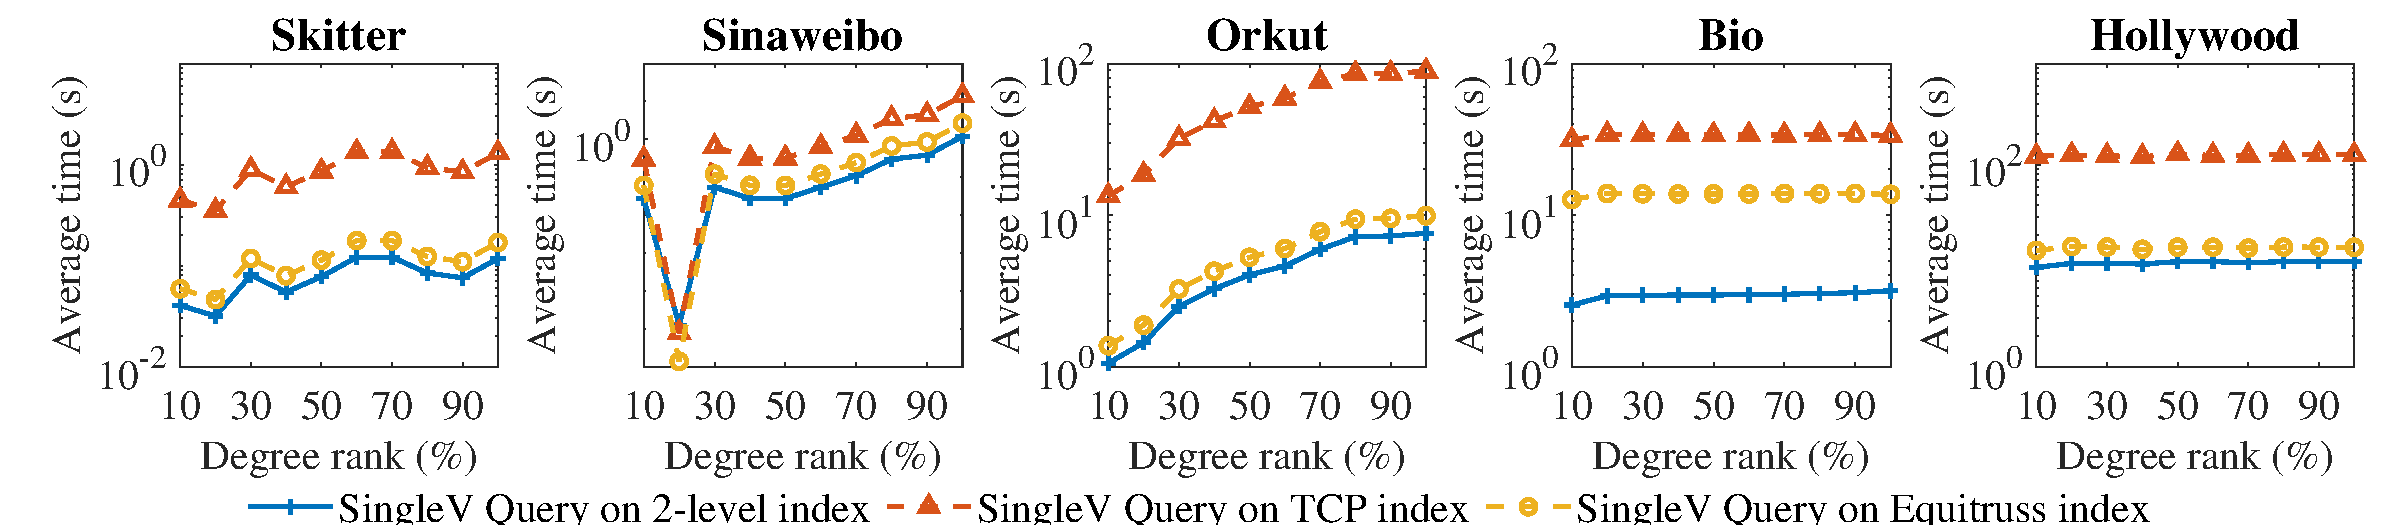
\includegraphics[width=0.9\linewidth, trim={0cm 0cm, 0cm, 0.3cm}, clip]{./figures/singlev_k_compare_small.pdf}
    \caption{Comparison of single-vertex k-truss community search of the \twolevelindex{}, the TCP index and the Equitruss index.}
    \label{fig:singlev_k_compare}
		\vspace{-0.3cm}
\end{figure*}

\begin{figure*}[h]
    \centering
    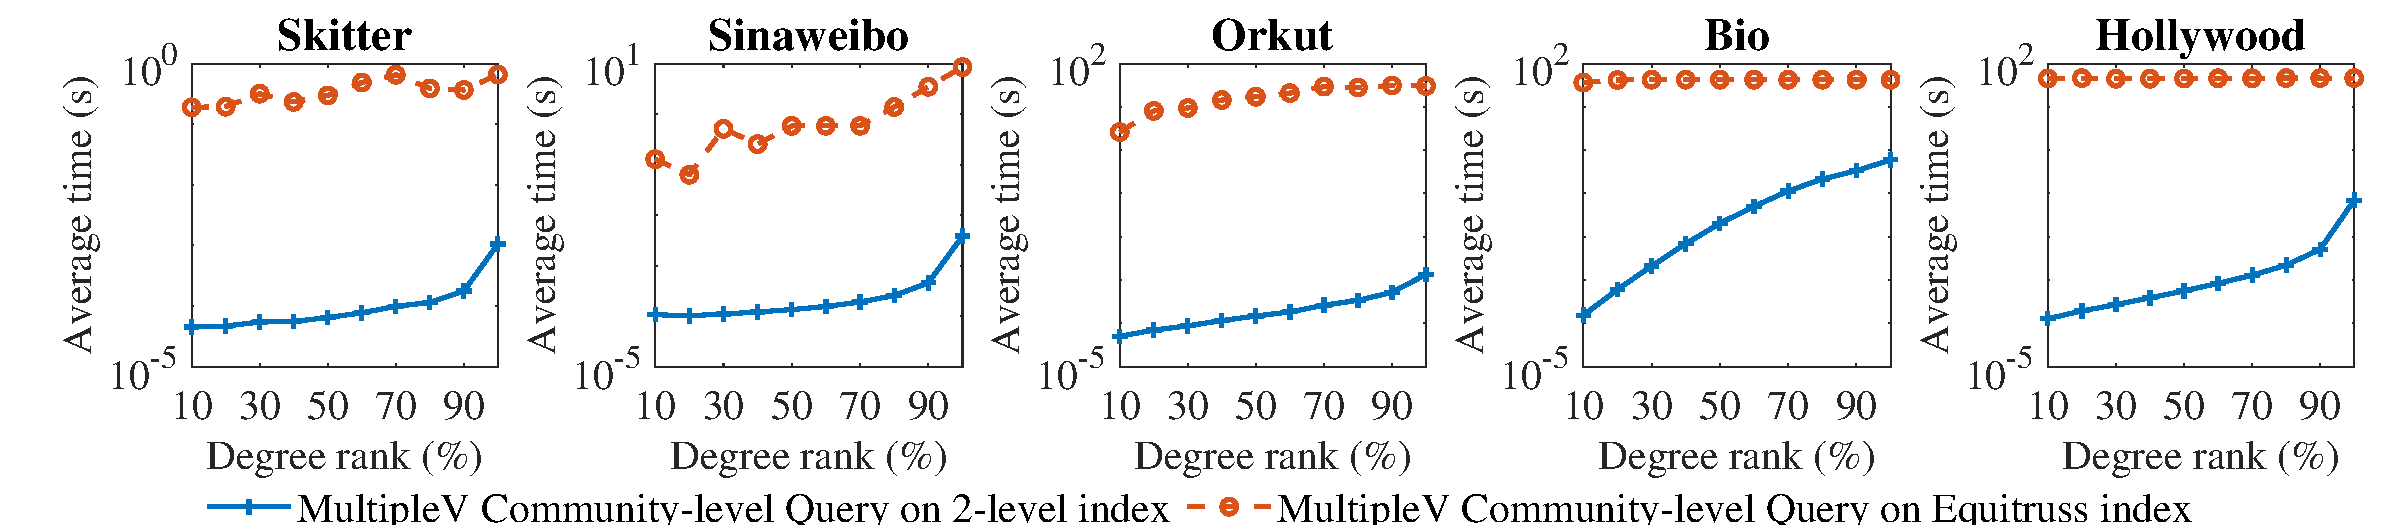
\includegraphics[width=0.9\linewidth, trim={0cm 0cm, 0cm, 0.3cm}, clip]{./figures/multiplev_k_compare_small.pdf}
    \caption{Comparison of multiple-vertex k-truss community-level query of the \twolevelindex{} and the Equitruss index.}
    \label{fig:multiplev_k_compare}
		\vspace{-0.3cm}
\end{figure*}

In this section, we evaluate our proposed index structure for various types of local k-truss community queries on real-world networks. We compare the \twolevelindex{} with the state-of-the-art solutions: the TCP index \cite{huang2014querying} and the Equitruss index \cite{akbas2017truss} for single-vertex k-truss community search (Section~\ref{eval_singlev_k_compare}) and multiple-vertex \probdef{} (Section~\ref{eval_multiplev}), respectively. All experiments are implemented in C++ and run on a Linux server with 2.2GHz CPUs and 256GB memory. 

\begin{table}
\caption{Datasets}
\label{table:datasets} 
\begin{threeparttable}
	\centering
		\begin{tabularx}{\linewidth}{c|*{5}{Y}} 
		\toprule
			Dataset & Type & $|V_{wcc}|$ & $|E_{wcc}|$ & $|{\triangle}_{wcc}|$ & $k_{max}$ \\
			\midrule
			%Wiki & Comm. & 2.4M & 4.7M & 9.2M & 53 \\ 
			%Baidu & Web & 2.1M & 17.0M & 25.2M & 31 \\
			Skitter & Internet & 1.7M & 11.1M & 28.8M & 68 \\ 
			Sinaweibo & Social & 58.7M & 261.3M & 213.0M & 80 \\ 
			%Livejournal & Social & 4.8M & 42.8M & 285.7M & 362 \\ 
			Orkut & Social & 3.1M & 117.2M & 627.6M & 78 \\
			Bio & biological & 42.9K & 14.5M & 3.6B & 799 \\
			Hollywood & Collab. & 1.1M & 56.3M & 4.9B & 2209 \\
			%Webuk & Web & 39.3M & 796.4M & & \\ 
			%Friendster & Social & 65M & 1.8B & & \\
			\bottomrule
			\end{tabularx}
			%\begin{tablenotes}
				%\item Number of vertices, edges, triangles and the maximum trussness ($k_{max}$) in the largest WCC. 
			%\end{tablenotes}
		\end{threeparttable}
		\vspace{-0.5cm}
\end{table}

We use five real-world graphs of different types shown in Table~\ref{table:datasets}. To simplify our experiments, we treat them as undirected, un-weighted graphs and only use the largest weakly connected component of each graph. %We also removed all the self edges in each graph. 
%We sort the graph according to their number of triangles as ktruss community highly relies on triangles in the graph. 
All datasets are publicly available from the Stanford Network Analysis Project (snap.stanford.edu) and the Network Repository (networkrepository.com).
We perform $10$-truss community queries and discard vertices with degrees less than $20$ as they normally do not belong to any $10$-truss community. 
%Because the query time heavily replies on the degree of query vertices, 
We uniformly partition the rest of vertices according to their degrees into 10 buckets and randomly select 100 sets of query vertices for each bucket.

%\subsection{Index construction}
%\label{eval_const}
%
%\begin{table}
		%\caption{Comparison of Index Construction}
		%\label{table:index_construction}
		%\centering
		%%\begin{tabular}{|c|c|ccc|ccc|} \hline 
		%%& Graph & \multicolumn{2}{|c|}{Index Size} & \multicolumn{2}{|c}{Index Time} \\
			%%\cline{3-6}
			%\begin{tabularx}{\linewidth}{c c *{6}{Y}}
			%\toprule
			%Graph & Decomp.
						%& \multicolumn{3}{c}{Index Time (Sec.)} 
						%& \multicolumn{3}{c}{Index Size (MB)} \\
			%\cmidrule(lr){3-5} \cmidrule(l){6-8}
			 %Name & Time (Sec.) & TCP & Equi & Our & TCP & Equi & Our \\ 
			%\midrule
			%%Wiki & 239 & 139 & 63 & 83 & 58 & 25 & 32 \\ 
			%%Baidu & 742 & 494 & 269 & 350 & 306 & 179 & 237 \\
			%Skitter & 151 & 167 & 151 & 139 & 139 & 240 & 193 \\ 
			%Sinaweibo & 10169 & 11048 & 5724 & 6871 & 2744 & 1390 & 1810 \\
			%%Livejournal & 2201 & 1313 & 795 & 1020 & 1129 & 585 & 844 \\ 
			%Orkut & 8731 & 7659 & 3609 & 5059 & 3302 & 1722 & 2479 \\
			%Bio & 13496 & 13964 & 6223 & 8874 & 393 & 177 & 289 \\
			%Hollywood & 12619 & 16620 & 4154 & 10182 & 1929 & 813 & 1276 \\ 
			%
			%%Wiki & 57.5 & 138.6 & 62.8 & 83.3 & 58.4 & 24.9 & 32.4 \\ 
			%%Baidu & 224.5 & 493.9 & 268.5 & 350.3 & 305.8 & 179.0 & 237.3 \\
			%%Skitter & 149.1 & 166.9 & 151.1 & 138.5 & 138.6 & 239.7 & 192.7 \\ 
			%%Sinaweibo & 4049.9 & 11047.6 & 5724.3 & 6870.7 & 2743.8 & 1390.0 & 1810.4 \\
			%%Livejournal & 627.6 & 1312.9 & 794.9 & 1020.0 & 1128.8 & 585.3 & 844.1 \\ 
			%%Orkut & 1769.8 & 7659.4 & 3609.1 & 5058.7 & 3301.6 & 1721.8 & 2479.0 \\
			%%Bio & 165.7 & 13963.9 & 6222.7 & 8873.6 & 393.1 & 176.6 & 289.4 \\
			%%Hollywood & 791.7 & 16619.7 & 4154.4 & 10181.7 & 1928.7 & 812.5 & 1276.3 \\ 
			%%Webuk & 13999 &   &  &  & \\ 
			%%Friendster & 32364 &   &  &  & \\
			%\bottomrule
		%\end{tabularx}
		%\vspace{-0.5cm}
%\end{table}
%
%In this section, we show the index size and index construction time of the \twolevelindex{} compared to the TCP index and the Equitruss index in Table \ref{table:index_construction}. 
%%Both indices are generated in memory and we show the size of the data structures that hold the index. 
%%We separate the truss decomposition time for all three methods. %so that the index construction time only shows how long it takes to generate a certain index with edge trussness provided. 
%We can see in Table \ref{table:index_construction} that the \twolevelindex{} has a construction time that is comparable with the Equitruss index and that both are faster than the TCP index. The index size of the \twolevelindex{} is smaller than the TCP index. %as there are no repeating edges stored in the index. 
%However, the Equitruss has the smallest index size since it only stores edge list of the original graph while the \twolevelindex{} also preserves the triangle connectivity inside k-truss communities. 
%%Note that if only \toplevelprob{} k-truss community queries are processed, the algorithm only needs to retrieve the top level index which has a much smaller size. 
%
%\subsection{Query performance}
%\label{eval_query_time}

%In this section, we evaluate the query time of k-truss community queries to show the effectiveness of the \twolevelindex{}. 
%As query time heavily relies on the degree of query vertices, we partition vertices for the experiments. 
%We discareds vertices Because only vertices with a degree of $k + 1$ can appear in a k-truss community with trussness of $k$. If we partition vertices uniformly by their degree and the graph has highly screwed degree distribution, then vertices in most of the partitions would have a too low degree to appear in a k-truss community. To show the performance of different algorithms on mining community structures in this kind of graphs, 


%\vskip 0.1in \noindent \textbf{Single vertex k-truss community search.}
\subsection{Single-vertex k-truss community search.}
\label{eval_singlev_k_compare}

We first evaluate the single-vertex k-truss community search performance and compare the query time with the TCP index and the Equitruss index. The results are shown in \autoref{fig:singlev_k_compare}. The \twolevelindex{} achieves the best average query time for all graphs. It has an order of magnitude speedup compared to the TCP index for all graphs, along with $5\%$ to $400\%$ speedup compared to the Equitruss index for all graphs. The speed up is linear as all three indices have the same time complexity to handle single-vertex k-truss community search queries. 
%Note that very low average query time (around $10^{-5}$ second) means that there is no vertex belonging to any k-truss community in that degree rank. 
The main reason why the \twolevelindex{} is faster than the TCP index is the avoidance of the expensive BFS search during query time. The reason behind the performance differences of the \twolevelindex{} and the Equitruss index on various graphs lies in the fact that the super-graph size of the \twolevelindex{} is much smaller, making it easier to locate target communities.

%\begin{figure}[h]
%\centering
%\subfigure[Number of vertices in super-graphs.\label{fig:graphsize_vertices}]{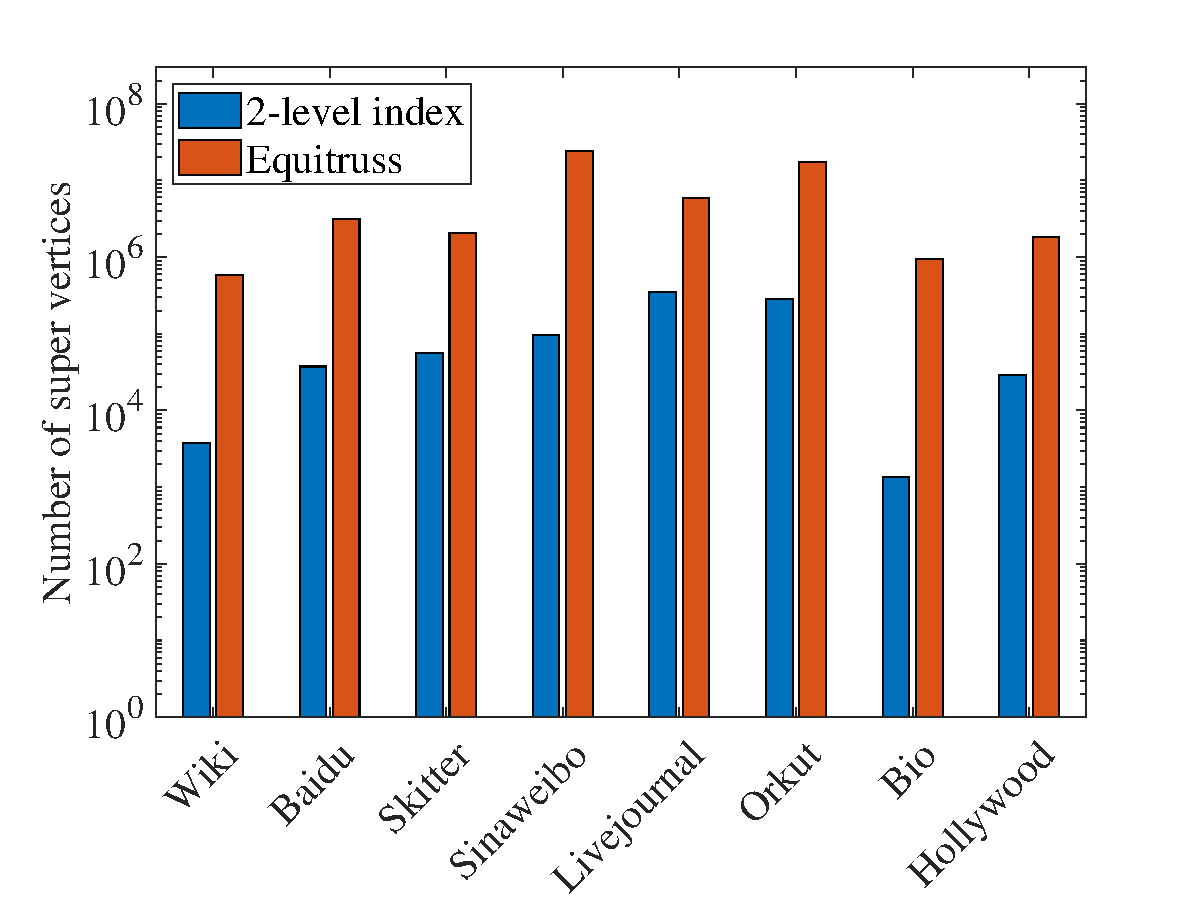
\includegraphics[width=0.45\linewidth]{./figures/super_node_compare.pdf}}
%\subfigure[Number of edges in super-graphs.\label{fig:graphsize_edges}]{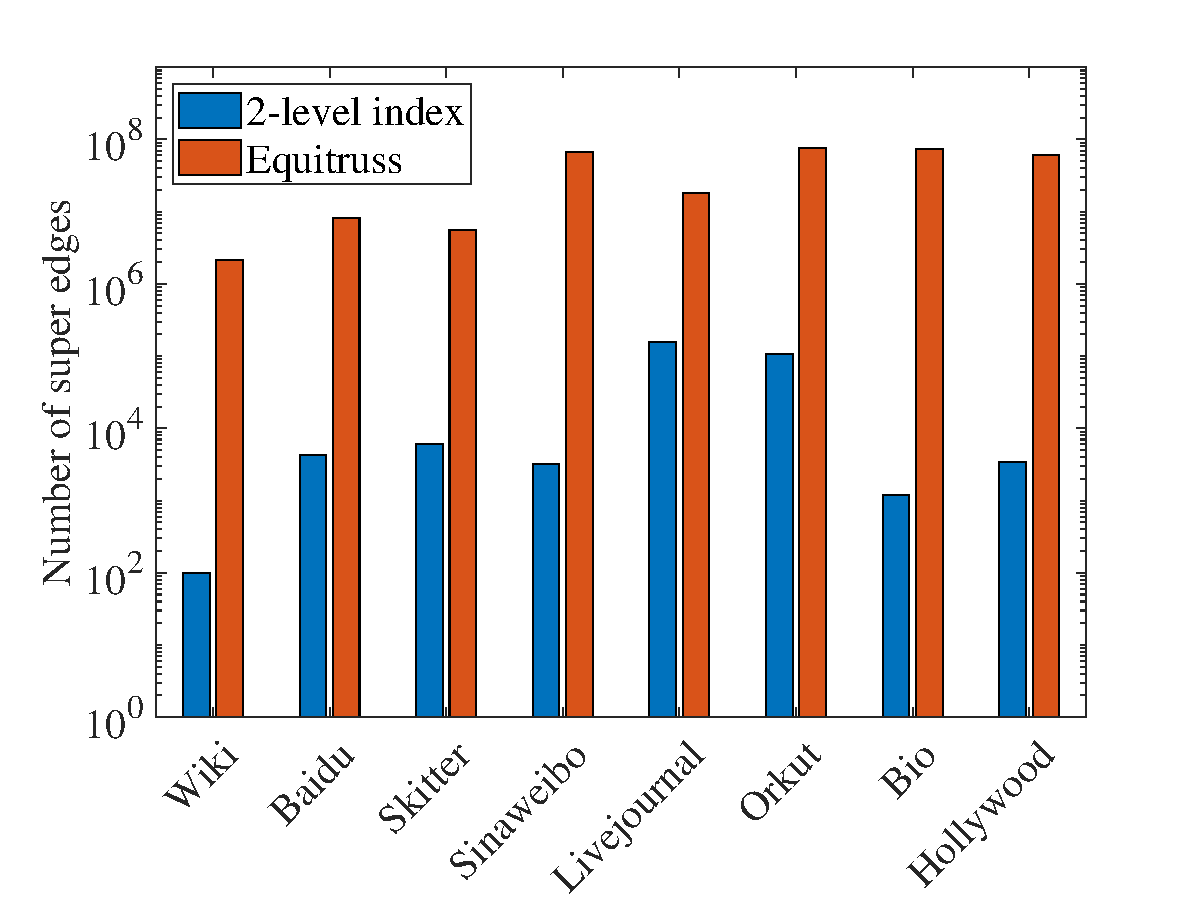
\includegraphics[width=0.45\linewidth]{./figures/super_edge_compare.pdf}}
%\caption{Super-graph size comparison of the \twolevelindex{} and the Equitruss index.}
%\label{fig:graphsize}
%\end{figure}
%
%\vskip 0.1in \noindent \textbf{Reason of performance difference.} The main reason that the \twolevelindex{} is faster than the TCP index is the avoidance of the expensive BFS search during query time. The reason for performance differences of the \twolevelindex{} and the Equitruss index on various graphs is less obvious given that they both search for target communities on a super-graph of the original graph and then collect edges belonging to the target community. The difference lies in the fact that vertices and edges in the super-graph of the two indices represent different subgraphs and their relations of the original graph. Each vertex in the \twolevelindex{} represents a single k-truss community while vertices in the Equitruss index only represents a fraction of a k-truss community. So one vertice in \twolevelindex{} may be split into several vertices in the Equitruss index. 
%
%We show the super-graph sizes of the \twolevelindex{} and the Equitruss index in \autoref{fig:graphsize}. We can see that the size of the super-graph of the Equitruss index is an order of magnitude larger than the super-graph of the \twolevelindex{}. The Equitruss index is slow while finding target communities due to the larger super-graph size. However, edge lists of a k-truss community can be more effectively retrieved as it is already stored in each super vertex. For the \twolevelindex{}, target communities are easier to identify, however, one need to iterate through the adjacent lists stored in super vertices to retrieve edges in the community. % and then convert vertices of the \inducedgraph{} back to their corresponding edges in the original graph. %Now it's not hard to understand the performance different on different real-world graphs, 

\subsection{Multiple-vertex k-truss community query.}
\label{eval_multiplev}

\begin{figure*}
    \centering
    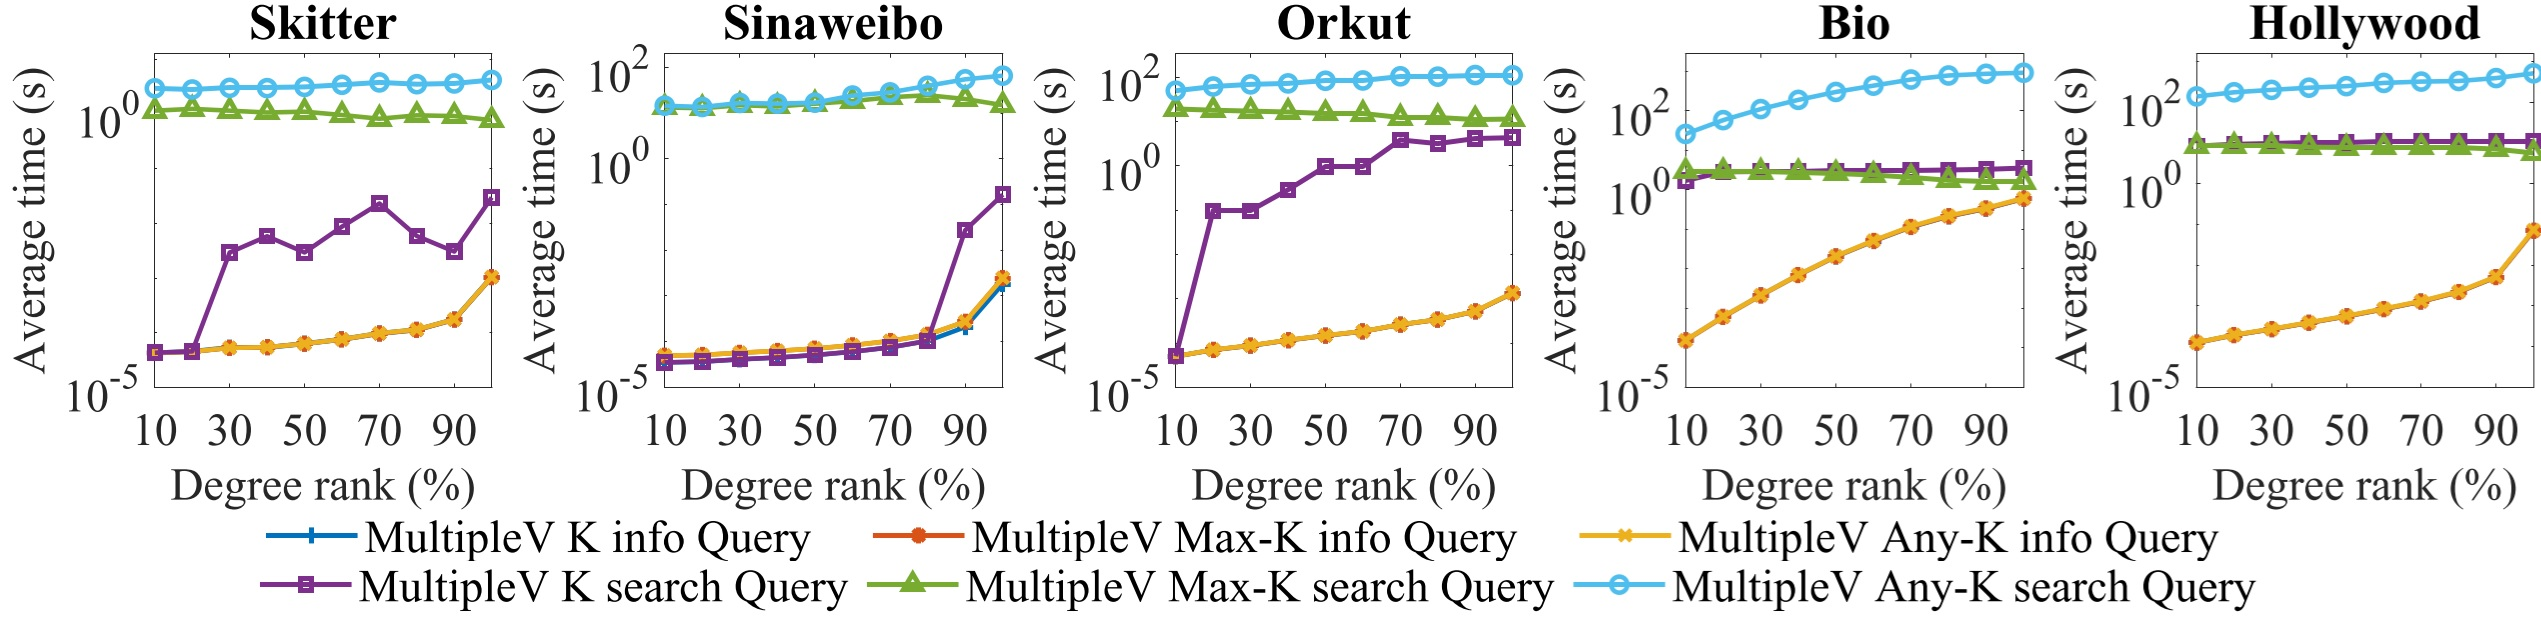
\includegraphics[width=0.9\linewidth, trim={0cm 0cm, 0cm, 0.2cm}, clip]{./figures/multiplev_3_info_query_small.jpg}
		\vspace{-0.2cm}
    \caption{Three types (k-truss, max-k-truss, any-k-truss) multiple-vertex ($3$) \toplevelprob{} k-truss community queries $vs.$ community search.}
    \label{fig:multiplev_3_info_query}
		\vspace{-0.5cm}
\end{figure*}

%\begin{figure*}[t]
    %\centering
    %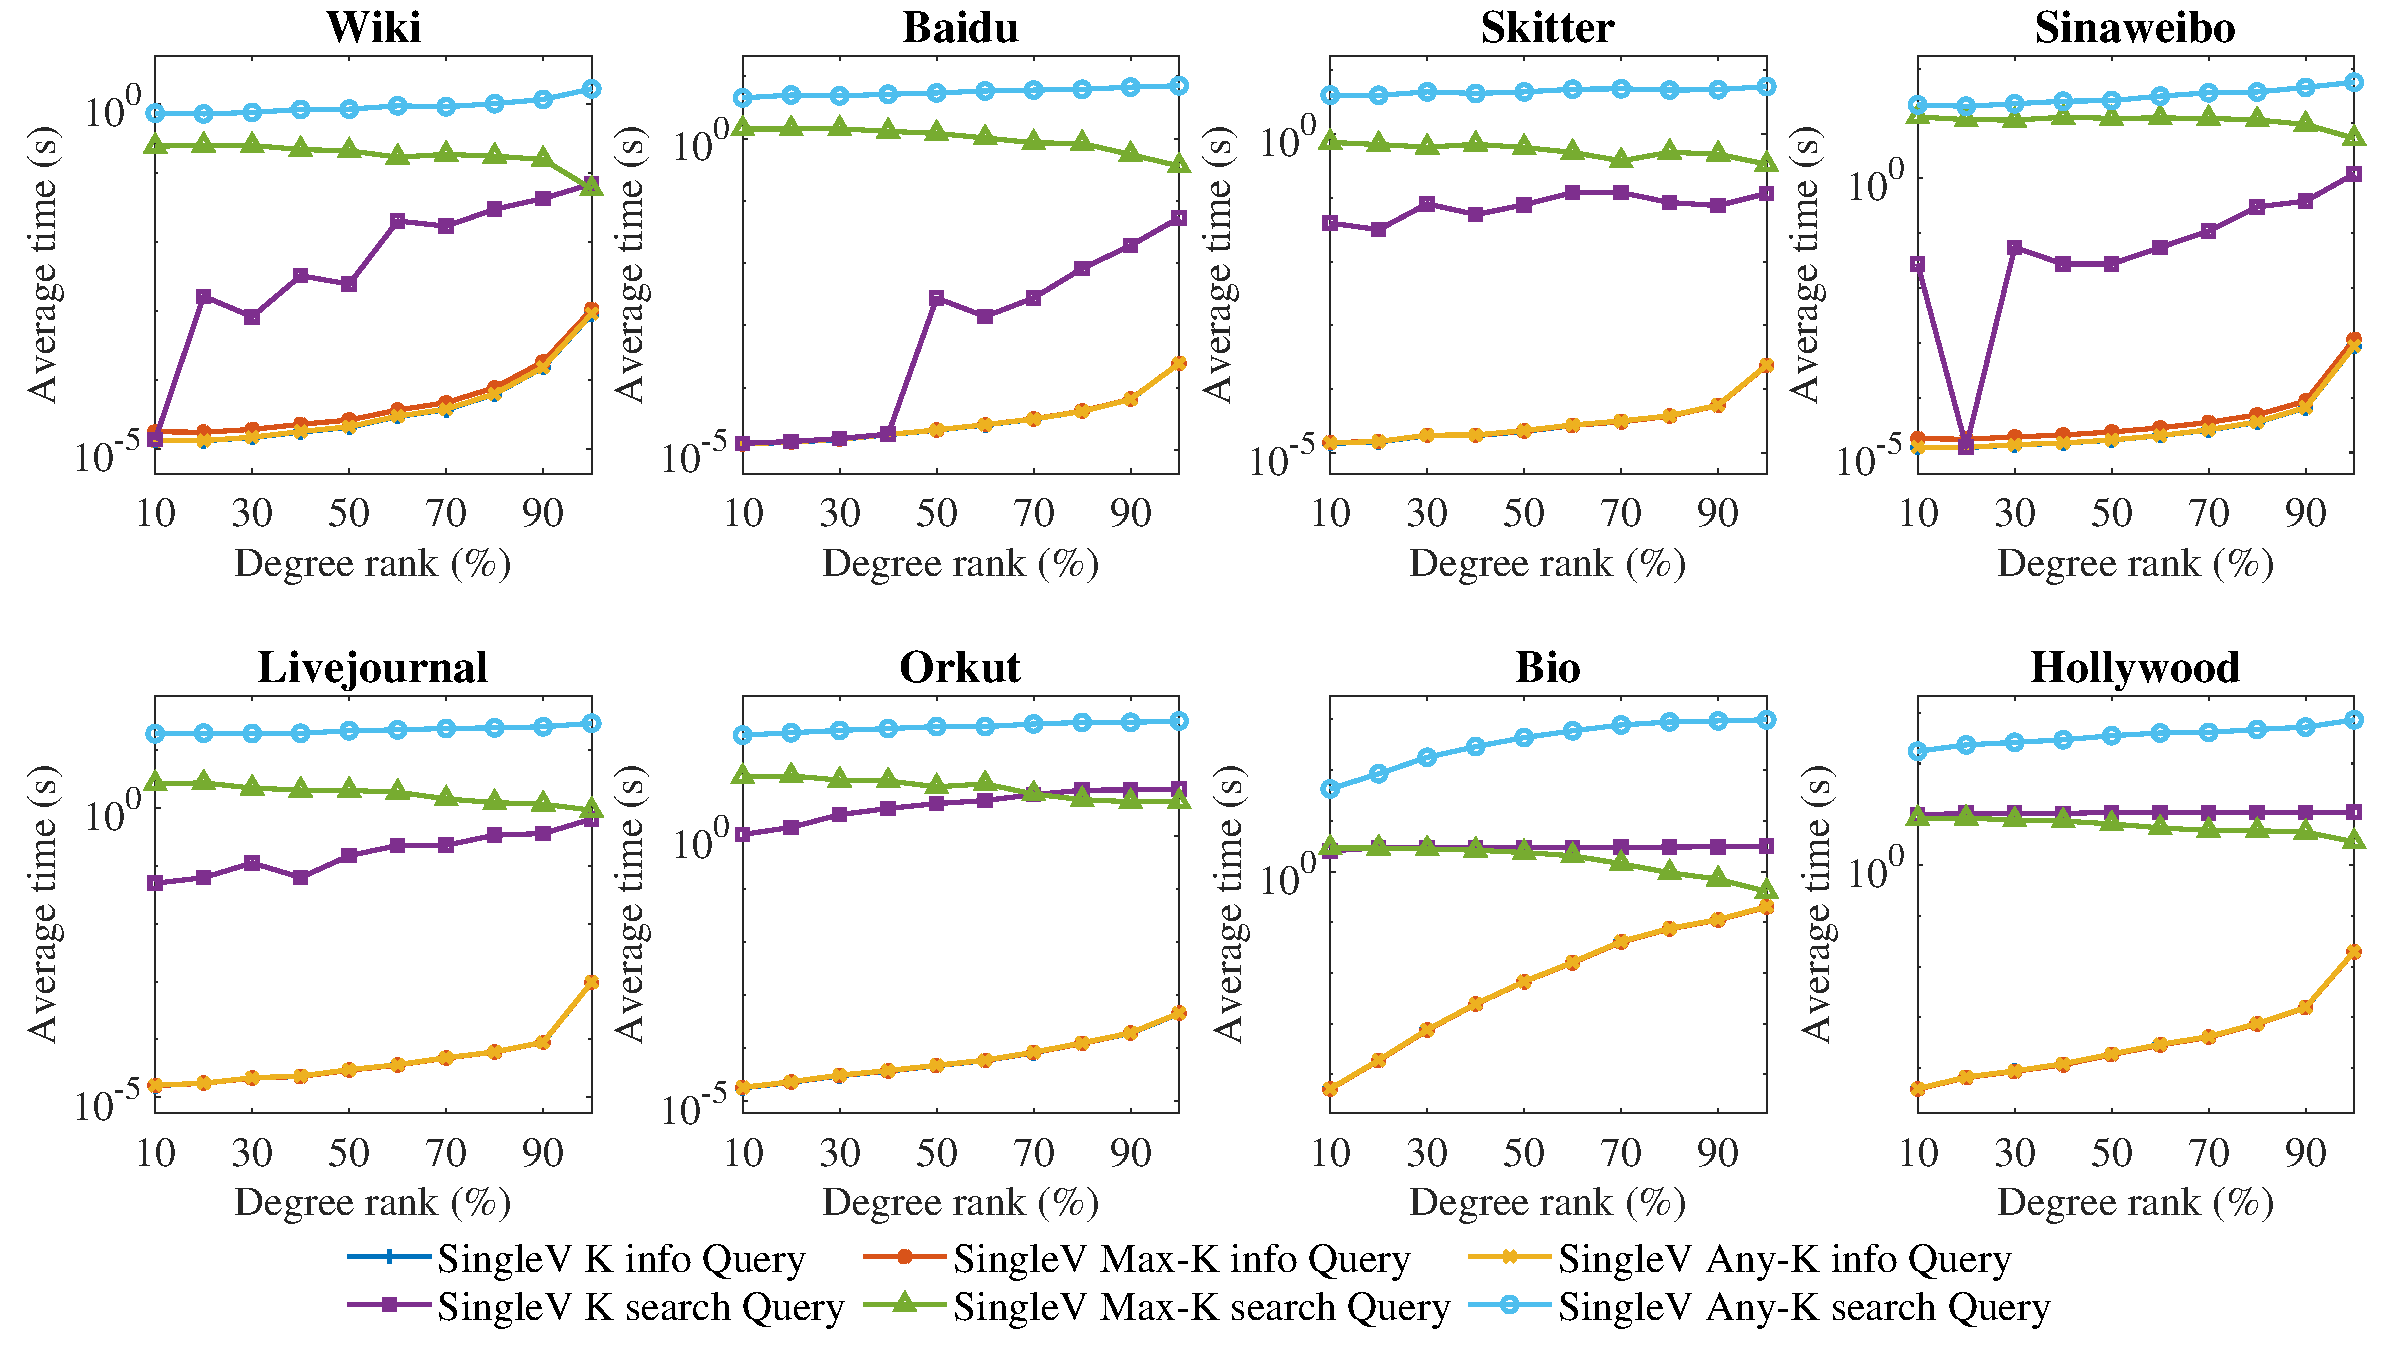
\includegraphics[width=0.8\linewidth]{./figures/singlev_info_query.pdf}
    %\caption{Three types (k-truss, max-k-truss, any-k-truss) of single-vertex \toplevelprob{} k-truss community query $vs.$ community search.}
    %\label{fig:singlev_info_query}
%\end{figure*}

%\begin{figure}[ht]
    %\centering
    %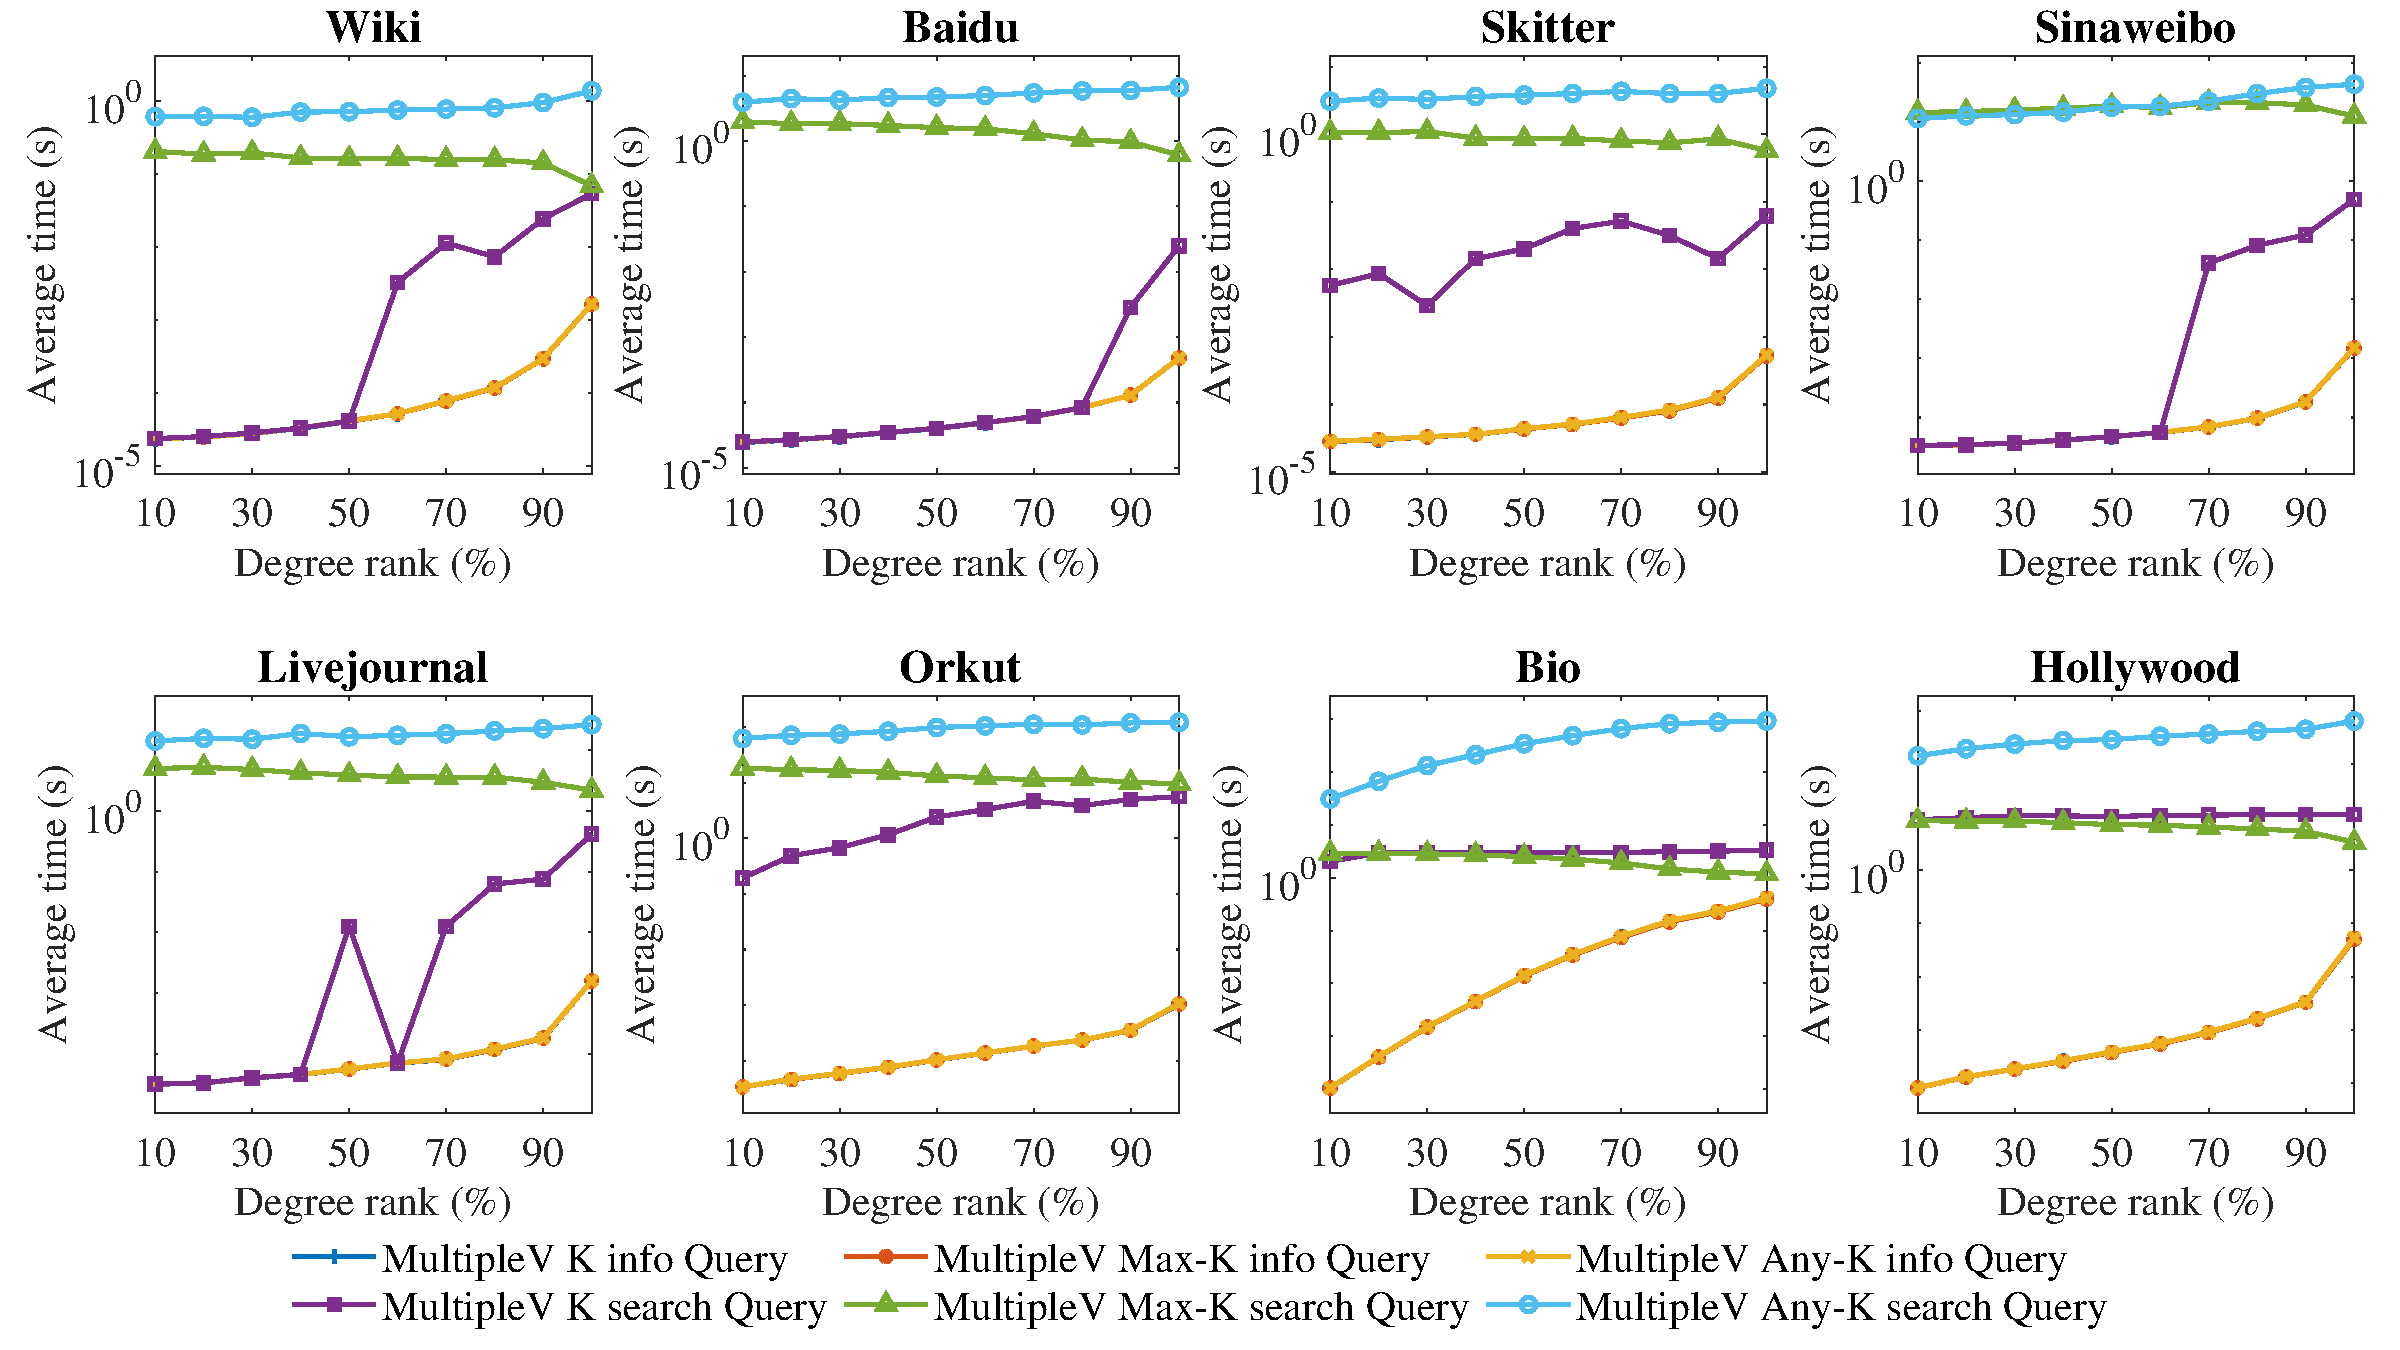
\includegraphics[width=\linewidth]{./figures/multiplev_2_info_query.pdf}
    %\caption{Single vertex query for exact truss community search.}
    %\label{fig:multiplev_2_info_query}
%\end{figure}

We first perform \toplevelprob{} multiple-vertex k-truss queries with both the \twolevelindex{} and the Equitruss index. We are not able to perform the same experiment on the TCP index as there is no easy modification that would enable it to support multiple-vertex queries. We can see in \autoref{fig:multiplev_k_compare} that the \twolevelindex{} outperforms the Equitruss index by several orders of magnitude. This clearly shows the difference between the two indices; the Equitruss index has a larger super-graph and is slower for \toplevelprob{} queries, where only the super-graph is required. %The performance difference shows that our \twolevelindex{} is quite suitable for \toplevelprob{} queries.

We then perform both the \toplevelprob{} and the \bottomlevelprob{} multiple-vertex queries with all three basic types of cohesiveness criteria, \ie k-truss, max-k-truss and any-k-truss. We show the results in \autoref{fig:multiplev_3_info_query}. The average time for \toplevelprob{} queries spans from $3.4$ x $10^{-5}$ second to $0.06$ seconds. Typically, the average time for community search queries is much higher than \toplevelprob{} queries (since one needs to access edge-level information), ranging from $0.03$ to $918.7$ seconds depending on the size of the target communities. Among all the three types of cohesiveness criteria, any-k-truss \bottomlevelprob{} queries usually take the longest query time. %as it needs to process the most k-truss communities. %The multi-hundred average run time comes from searching all truss communities that contain a query vertex (any-k-truss query) with a very high degree in the densest graph (bio). %The fast query time of \toplevelprob{} queries makes it an excellent candidate for applications that require community-relation information such as whether a set of vertices belong to the same k-truss communities without digging into the details of any k-truss community. 

%\subsubsection{K-truss query $vs.$ max-k-truss query $vs.$ any-k-truss query.}
%\label{eval_k_type_compare}
%
%%\vskip 0.1in \noindent \textbf{K-truss query $vs.$ max-k-truss query $vs.$ any-k-truss query.} 
%We can also see in \autoref{fig:singlev_info_query} and \autoref{fig:multiplev_3_info_query} any-k-truss community search queries always have the highest average run time because it searches all the possible truss communities to which the query vertex/vertices belong. We can also see that k-truss community search queries usually have much smaller average run time than max-k-truss community search queries. 
%%Is it because the index are more effective for k-truss community search query? Not really. 
%%When checking the search result data, we find 
%It is because that many k-truss queries fail to find a truss community as the query vertex/vertices do not belong to any truss community with the specified $k$, which is $10$ in our experiments. However, this problem is less severe for max-k-truss queries. Max-k-truss queries can always find a target community as long as the query vertex/vertices belong to any truss community. In most cases, max-k-truss queries can provide more useful information for applications that do not have much knowledge of the community structure in the underlying graph.
%
%Another interesting trend is that as the degree of query vertex increases, the average run time for k-truss and any-k-truss community search queries increases, the average run time for max-k-truss queries decreases. The trend is caused by different reasons for three types of query. For k-truss queries, the average query time increases as the query vertex degree increases because that it is more likely to find a target k-truss community with the specified $k$, which is $10$ in our experiments. For max-k-truss queries, the average query time decreases as the query vertex degree increases because that target truss communities have higher trussness and smaller size. For any-k-truss queries, because the k-truss communities have hierarchical structures, more truss communities will be discovered by a query so that the average query time increases when the query vertex degree increases.

%\subsection{\BottomLevelProb{} Query Analysis}
%\label{eval_bottom_analysis}
%
%%\begin{figure}[h]
%%\centering
%%\subfigure[Boundary search.\label{fig:boundary}]{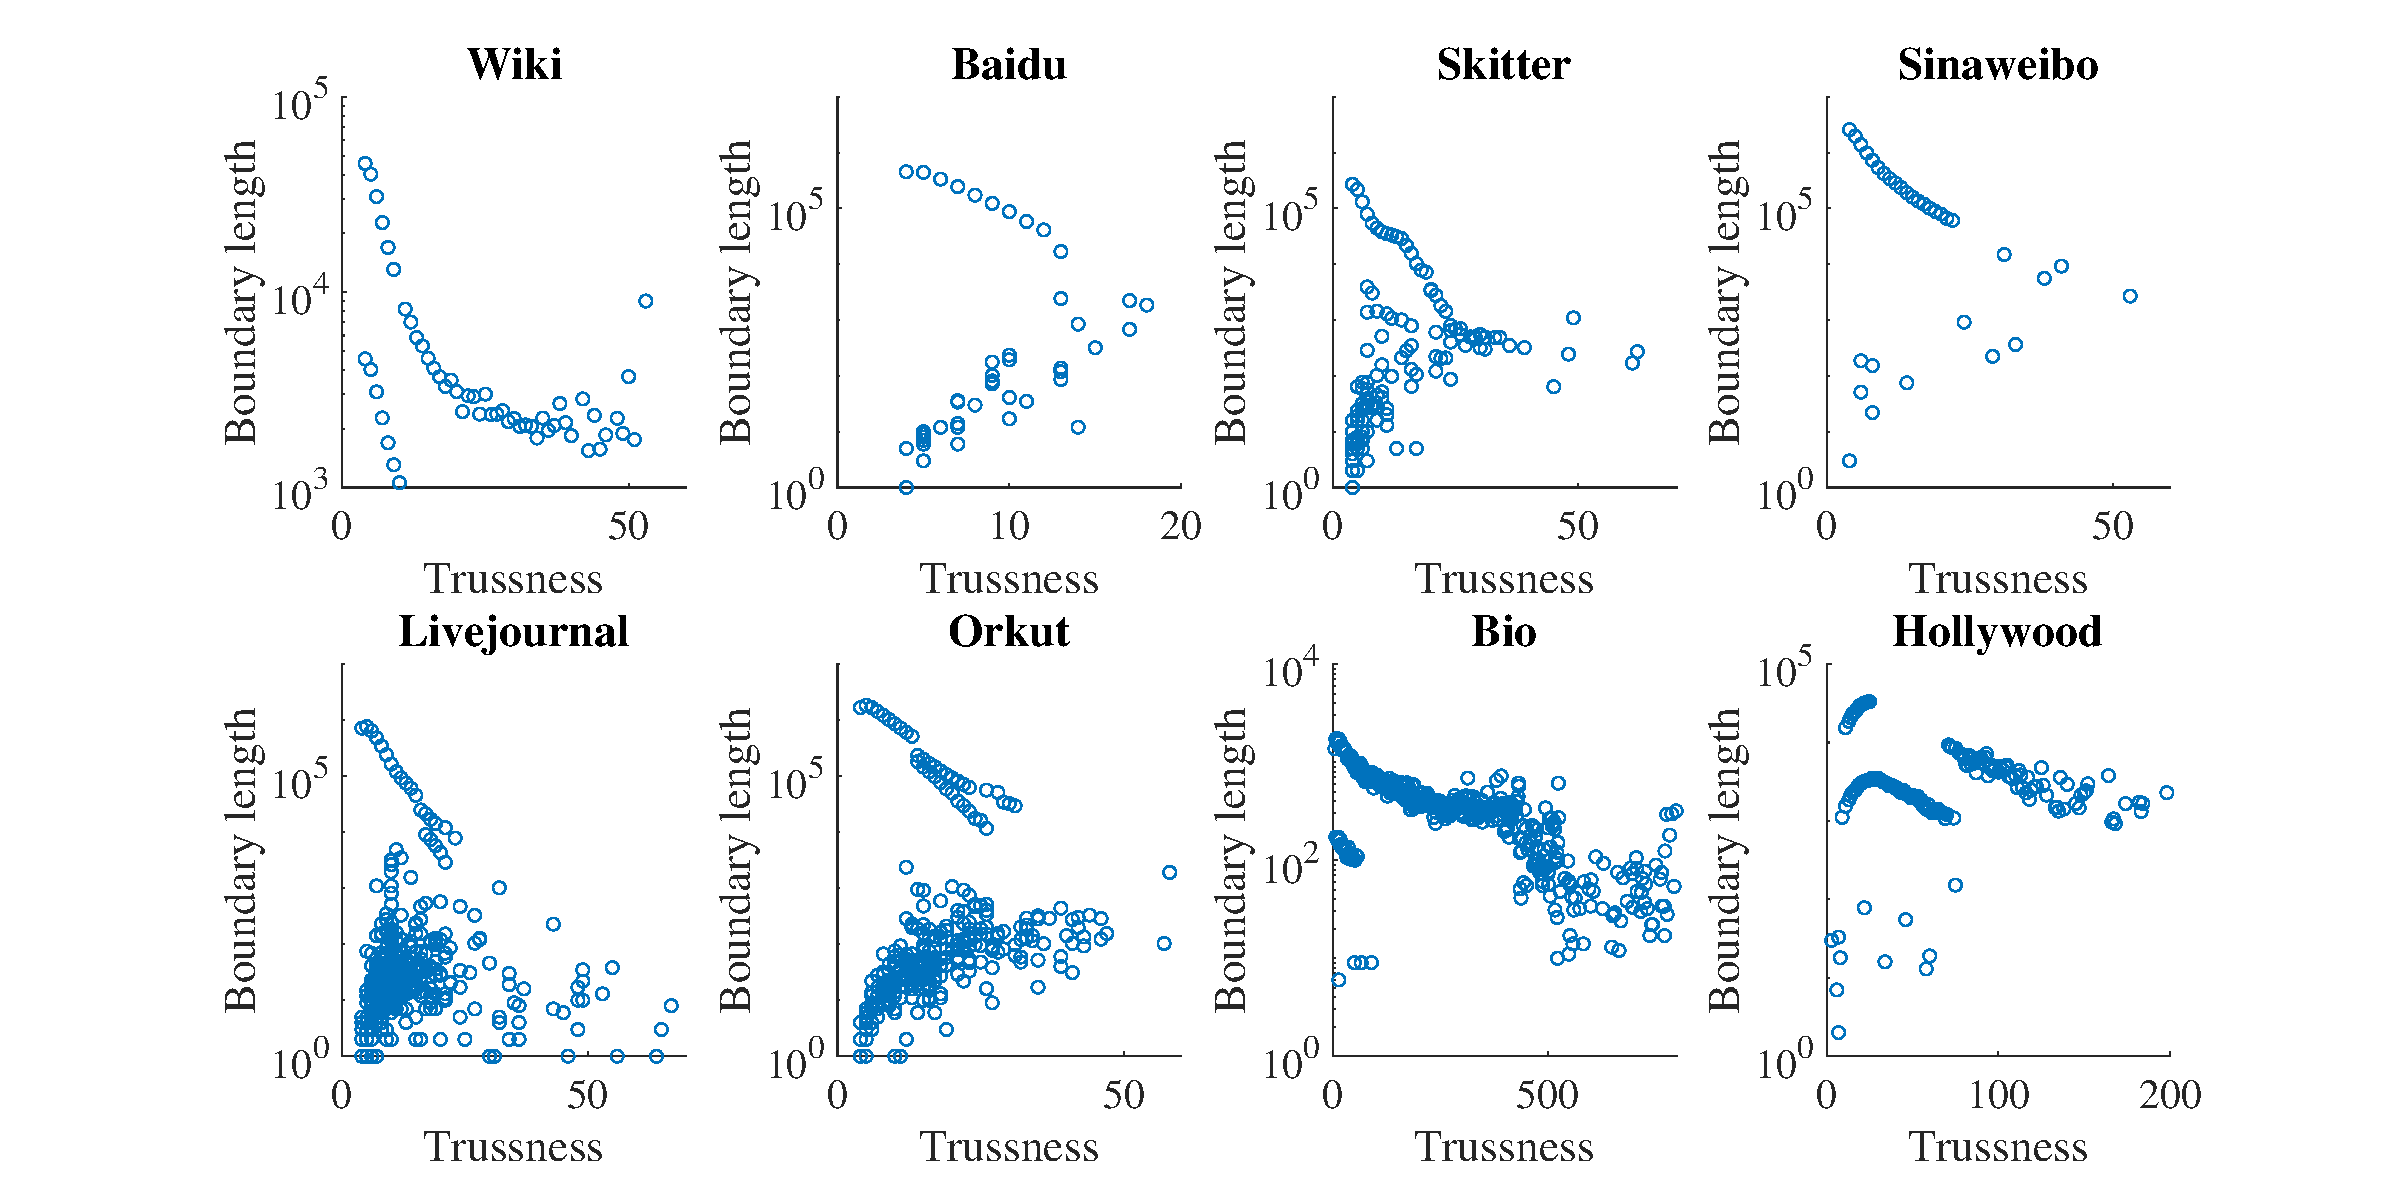
\includegraphics[width=0.78\linewidth]{./figures/boundary_size.pdf}}
%%\subfigure[Maximim triangle connected path.\label{fig:path}]{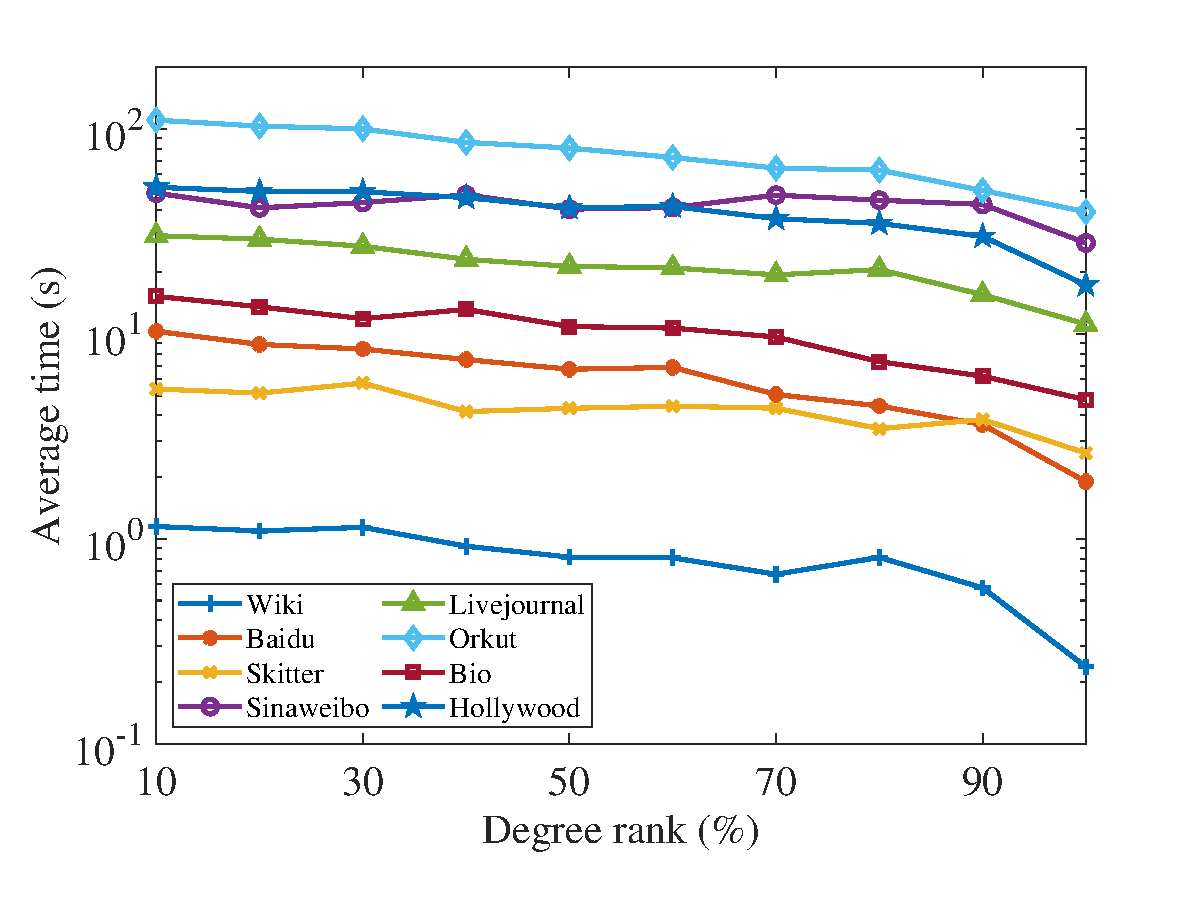
\includegraphics[width=0.18\linewidth]{./figures/path.pdf}}
%%\caption{Queries inside communities.}
%%\label{fig:inside_query}
%%\end{figure}
%
%\subsubsection{K-truss community boundary search.}
%
%\begin{figure}[ht]
    %\centering
    %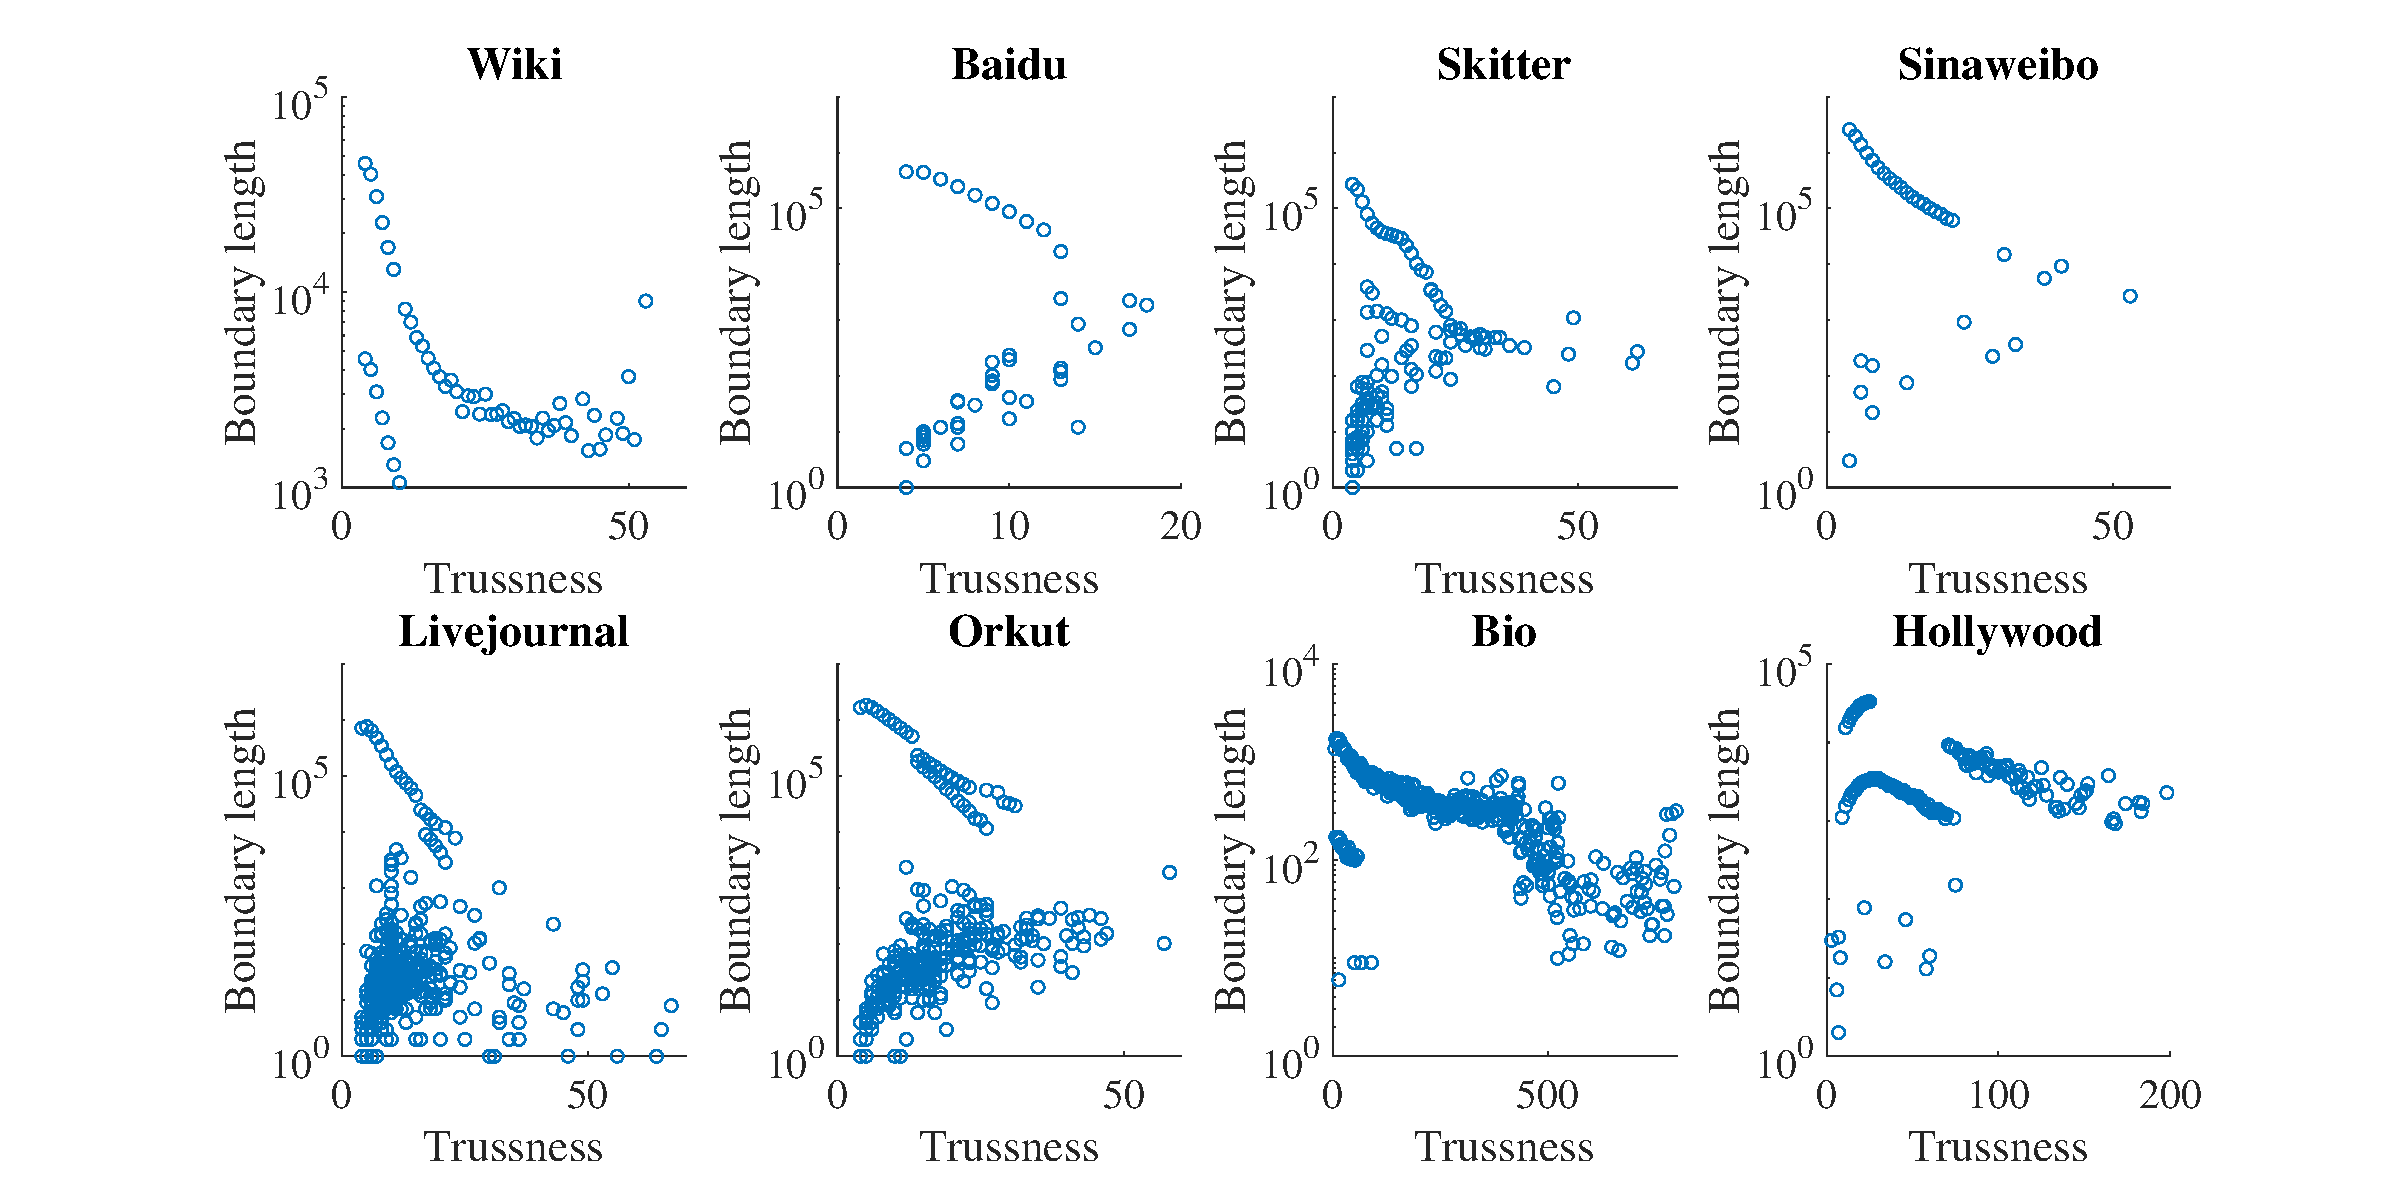
\includegraphics[width=\linewidth]{./figures/boundary_size.pdf}
    %\caption{Randomly sampled boundary length for k-truss communities with different trussness.}
    %\label{fig:boundary}
%\end{figure}
%
%%\vskip 0.1in \noindent \textbf{Boundary search.} 
%We randomly select $1000$ query vertices from various degree buckets and perform the boundary search for the k-truss community with highest trussness that contains each query vertex and the trussness of the community and their boundary length in \autoref{fig:boundary}. We can see that in many graphs there is a huge k-truss community of size several magnitude larger than other smaller k-truss communities. This community usually have a hierarchical structure, \ie larger k-truss communities with low trussness contain smaller k-truss communities with high trussness. \autoref{fig:boundary} also shows that the upper bound of the boundary length of k-truss communities decreases as the trussness increases. The main reason for this is that sizes of high trussness k-truss communities are usually smaller than sizes of low trussness k-truss communities. However, the lower bound of the boundary length of k-truss communities increases as the trussness increases. The reason is that there are many small-size k-truss communities which are triangle connected to very few other k-truss communities, \ie they are like isolated islands of the graph and many of them haven't formed a hierarchical structure. 
%
%\subsubsection{Triangle connected maximin path search.}
%
%\begin{figure}[ht]
    %\centering
    %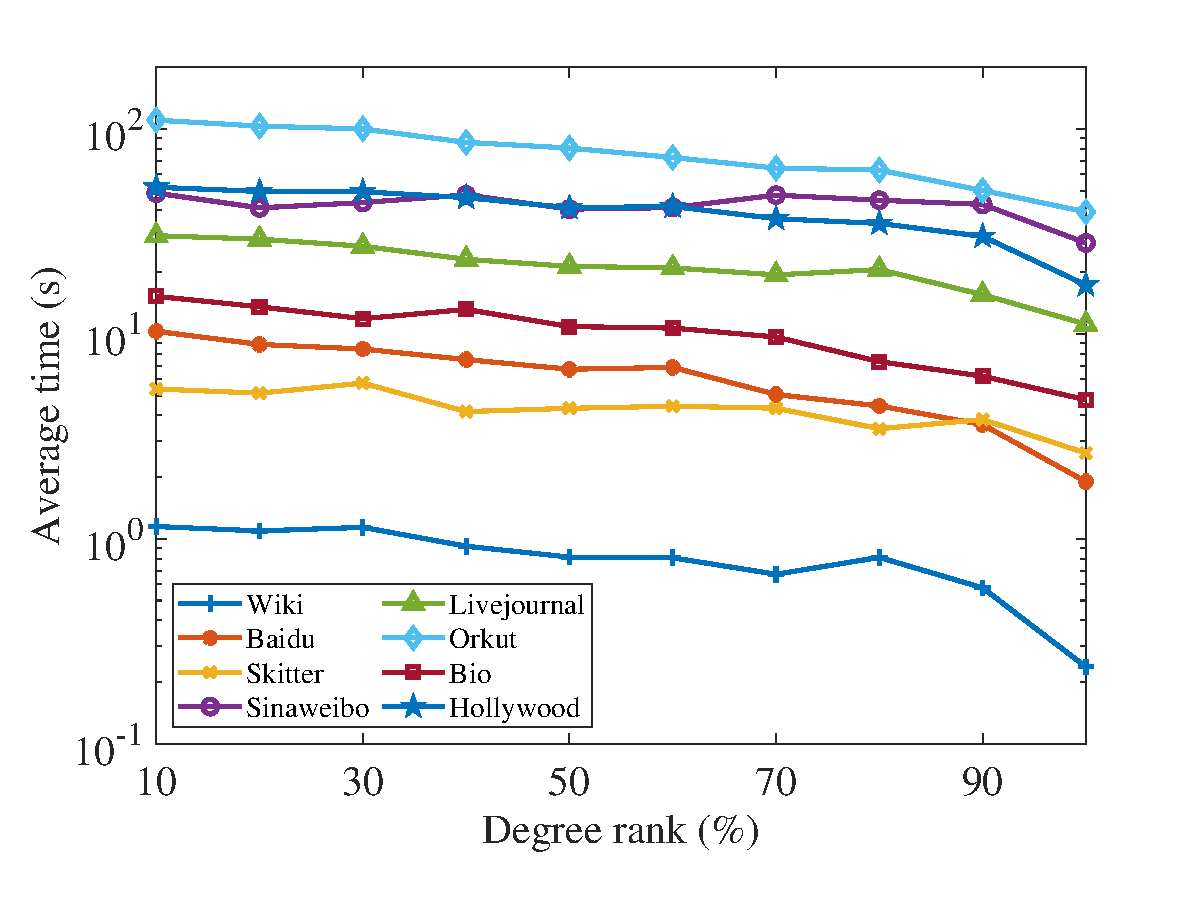
\includegraphics[width=0.5\linewidth]{./figures/path.pdf}
    %\caption{Average query time for triangle connected maximim path search.}
    %\label{fig:path}
%\end{figure}
%
%We randomly select $1000$ pair of vertices from various degree buckets and show the average query time for the triangle connected maximin path search with them in \autoref{fig:path}. 
%%\vskip 0.1in \noindent \textbf{Maximin path search.} 
%The figure clearly shows that as the degree of vertex increases, the query time decreases. The reason is that for a pair of vertices with high degree, it is more likely that they belong to the same k-truss community with higher trussness and smaller size. So there is no surprise that the query vertices are closer to each other and a triangle connected maximim path between them tends to be shorter. We notice that the triangle connected maximin path search have much higher average query times for the same graph than k-truss community search because it needs to run a BFS traversal inside a target community which is very time-consuming.
